When the Rubik's Cube was globally released in 1980, it became an instant success, selling around 200 million units by the end of 1983 \cite{unitssold}. The Rubik's Cube also quickly became a popular subject of research for computer scientists, in part due to the massive 43 quintillion possible states \cite{states} that the cube can be in. Many different algorithms were designed to try and solve the cube in as few a number of moves as possible, but it wasn't until 1997 that Richard E. Korf published a paper \cite{korf} describing a method to solve the Rubik's Cube optimally (the shortest possible number of moves to solve any given cube state) by using large lookup tables called pattern databases \cite{patterndatabases} as a heuristic function to guide an IDA* search algorithm. 

Another key area that researchers focused on had to do with a concept called "God's Number", which is the maximum number of moves needed to solve the cube from any given state. Throughout the '90s and '00s, researchers were able to tighten the bounds on the God's Number for the Rubik's Cube, until in 2010 it was finally proved that the cube's God's Number is exactly 20 \cite{godsnumber}. This means that for any optimal solver (such as Korf's algorithm), the solver will always be able to find a solution in 20 moves or less (given enough time to find the solution).

\begin{figure}[h]
    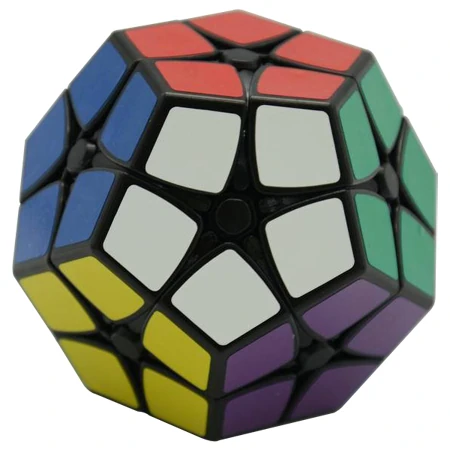
\includegraphics[width=0.4\textwidth]{kilominx}
    \centering
    \caption[An image of a Kilominx.]{An image of a Kilominx\footnotemark.}
\end{figure}

\footnotetext{This image is taken from the \href{https://speedcubesolving.fandom.com/wiki/Kilominx}{"Kilominx"} article on the \href{https://speedcubesolving.fandom.com}{Speed Cube Solving wiki} at \href{https://www.fandom.com/}{Fandom} and is licensed under the \href{https://creativecommons.org/licenses/by-sa/4.0/}{Creative Commons Attribution-Share Alike License}.}

The widespread success of the Rubik's Cube also led to the creation of a number of different variants of the puzzle, each working similarly to the Rubik's Cube but of different shapes and sizes. The Kilominx is one of these variants, part of the larger "minx" family of dodecahedron-shaped puzzles. The Kilominx is a 2x2 dodecahedral puzzle with 12 faces and 20 cubies (individual cube-shaped elements of the puzzle). Although some research has been done on tightening the bounds of its God's Number \cite{kilominxgodsnumber}, no optimal solver has previously been created for the puzzle.

The main goal for this project was to create an optimal solver for the Kilominx, applying similar principles to Korf's algorithm for the Rubik's Cube -  using pattern databases to guide an IDA* search algorithm. An additional goal was to use the solver to help increase the lower bound of Kilominx's God's Number by trying to find an optimal solution of a greater number of moves than the current lower bound.

\section{Project Objectives}
Below is a list of the objectives for this project, which are grouped based on their priority. It should be noted that the priorities of the objectives are slightly different to the original priorities as outlined in the DOER - these were updated after the project was started to better reflect which objectives were the most important for the project.

\textbf{Primary Objectives:}
\begin{itemize}
    \item Create an optimal solver for the Rubik's Cube, using an IDA* search algorithm and pattern databases (as described in Korf's paper).
    \item Create an optimal solver for the Kilominx, using the same principles as used in the Rubik's Cube solver.
\end{itemize}

\textbf{Secondary Objectives:}
\begin{itemize}
    \item Use the solver to tighten the bounds of the Kilominx's God's Number.
    \item Create a simple GUI to allow users to interact with a Rubik's Cube and Kilominx, and use the solvers to find optimal solutions for both puzzles.
\end{itemize}

\textbf{Tertiary Objectives:}
\begin{itemize}
    \item Survey users about their experience using the GUI and solver to gather feedback on its ease of use.
    \item Investigate better ways to allow users to input a Kilominx state into the solver (e.g. with computer vision).
\end{itemize}